% 
%	Jan Kechel
%	
%
\documentclass[landscape]{slides}
\usepackage{color,german}
\usepackage{graphicx}
%
\begin{document}
%
\title{TeamFound\\Infrastrukturen zur Open Source Softwareentwicklung\\Technische Universit"at Berlin}
\author{A. Bachmann, J. Heese, J. Kechel, M. Klink}
\date{WS 2005/2006}

%
\maketitle%
%
%%
\begin{slide}{Gliederung}

\textbf{1. Einf"uhrung}\\
Idee, Zielsetzung, Architektur-"Uberblick, Interface

\textbf{2. Implementation Server}\\
Architektur, Request/Response , Datenstruktur 

\textbf{3. Implementation Clients}\\
Web-Client, Firefox Toolbar, IE Toolbar

\textbf{4. Ablauf}\\
Beginn, 2005, 2006, Aktueller Stand

\textbf{5. Pr"asentation}
\end{slide}
%
%
%
%
\begin{slide}{1.1 Was ist TeamFound?}\\

TeamFound ist...

\begin{itemize}
\item eine Suchmaschine
\item nicht mit einem eigenen Crawler ausger"ustet
\item nicht auf einem lokalen Computer sondern "uber einen Webserver erreichbar
\item daher von beliebig vielen Menschen benutzbar
\end{itemize}

\end{slide}
%
\begin{slide}{1.2 Was bringt TeamFound?}\\

Einfacher UseCase:

\begin{itemize}
\item Alice will ihre E-Mails verschl"usseln und sucht nach geeigneter Software
\item Alice findet GnuPG und speichert ihr Suchergebnis in TeamFound
\item Bob sucht ebenfalls nach einer solchen L"osung
\item Bob findet sofort den Eintrag von Alice im TeamFound
\end{itemize}
\end{slide}
%
\begin{slide}{1.2 Oder anders}\\

Denkbar auch f"ur:

\begin{itemize}
\item Alle m"oglichen Teams mit Rechercheaufwand (Open-Source, Softwareentwicklung, ...)
\item Studenten \& Recherche f"ur Vorlesungen
\item Lose Gruppen mit bestimmten Themen (Angeln, Ski-Fahren,...)
\end{itemize}
\end{slide}

\begin{slide}{1.4 Wie funktioniert TeamFound?}\\

\begin{itemize}
\item Der TeamFound-Server definiert nur ein einfaches Protokoll

\item Anfrage-Parameter werden in Form von HTTP GET Variablen "ubertragen
\end{itemize}
\begin{verbatim}
http://teamfound:8080/tf/tf?keyword=teamfound
&want=xml&version=2&command=search&category=1
\end{verbatim}


\end{slide}

\begin{slide}{1.4 Wie funktioniert TeamFound? (2)}\\

Beispiel Antwort
\begin{verbatim}
<response>
  	<interface-version>2</interface-version>
  	<return-value>0</return-value>
  	<return-description>OK</return-description>
  	<search>
    		<keywords>
      			<word>teamfound</word>
    		</keywords>
\end{verbatim}
\end{slide}

\begin{slide}{1.4 Wie funktioniert TeamFound? (3)}\\

\begin{verbatim}
    		<result>
      			<count>30</count>
      			<found>
        			<url>http://teamfound.berlios.de</url>
        			<title>TeamFound - share your search results</title>
        			<incategory>0</incategory>
      			</found>
    		</result>
  	</search>
</response>
\end{verbatim}
\end{slide}

%
%
%
\begin{slide}{2.1 Architektur des Servers}\\
\begin{center}
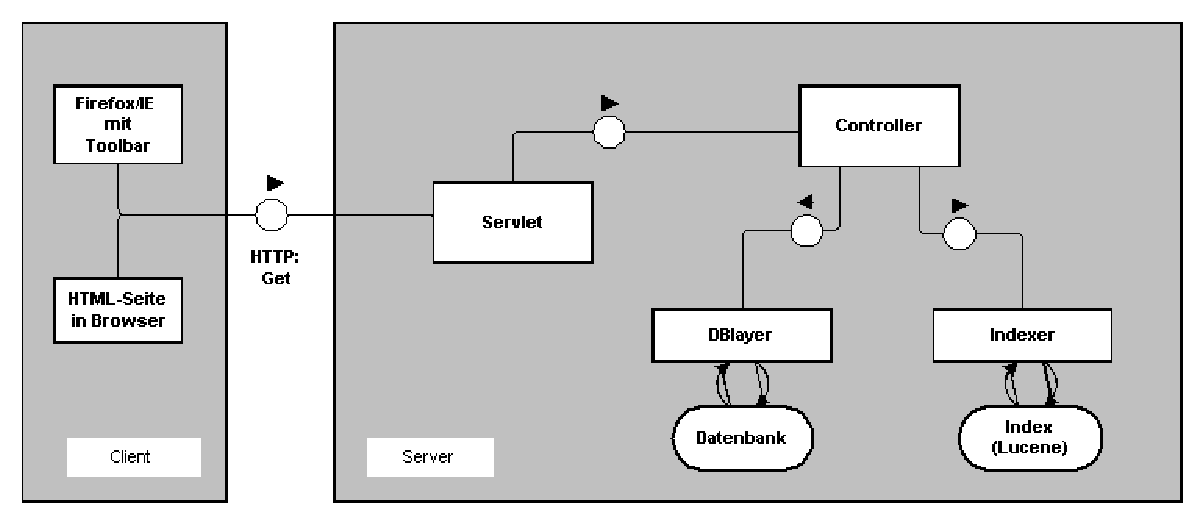
\includegraphics{bilder/aufbau2.eps}
\end{center}
\end{slide}
%
\begin{slide}{2.2 Request/Response }\\
\begin{itemize}
\item Antworten vom Server
\begin{itemize}
\item HTML-Seite: die direkt im Browser angezeigt wird
\item XML-File: wird von der Toolbar interpretiert
\end{itemize}	
\end{itemize}
\end{slide}
%
\begin{slide}{2.2 Beispiel Request}\\
\end{slide}
%
\begin{slide}{2.3 Lucene Index}\\
\begin{itemize}
\item Wichtige Komponenten von Apache Lucene:
\begin{itemize}
\item Document und Field
\item Analyzer
\item Query
\end{itemize}
\end{itemize}
\end{slide}

%	
\begin{slide}{2.4 Datenstruktur}\\
\begin{center}
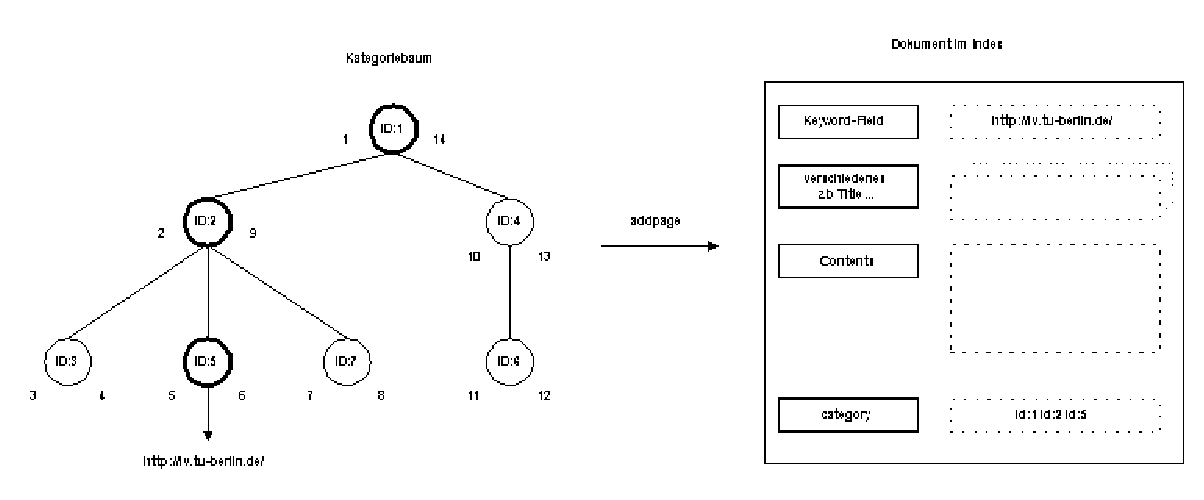
\includegraphics[width=17cm]{bilder/katstruktur.eps}
\end{center}
\end{slide}
%
%
%
\begin{slide}{3.1 Web-Client}\\

Web-Client ..

\end{slide}
%
\begin{slide}{3.2 Firefox Toolbar}\\
FF-Toolbar ..
\end{slide}
%
%
%
\begin{slide}{3.3 Internet Explorer Toolbar}\\
IE Toolbar ..
\end{slide}
%%
%%
%
\begin{slide}{4.1 Projektverlauf}\\
Das Projekt hat damit begonnen, ..
\end{slide}
%
%
%
\begin{slide}{5.1 Pr"asentation}\\
Pr"asentation
\end{slide}
%
%
%
%
\begin{slide}{}
The End
\end{slide}
%%%%%%%%%%%%%%%%%%%%%%%
\end{document}
